\documentclass[11pt,a4paper]{article}
\usepackage[margin=2.5cm]{geometry}
\usepackage{amsmath,amssymb}
\usepackage{graphicx}
\usepackage{booktabs}
\usepackage{caption}
\usepackage{float}
\usepackage[hidelinks]{hyperref}
\usepackage{microtype}
\usepackage{enumitem}
\newcommand{\code}[1]{\texttt{#1}}
\hypersetup{
  pdftitle={Problem Set 3 - Statistical Learning and Data Analytics for
            Transportation Systems},
  pdfauthor={Mohd Zamin Quadri},
  pdfsubject={Neural networks, reinforcement learning and convolutions},
  pdfkeywords={},
  pdfcreator={},
}

\title{\vspace{-1.5cm}Statistical Learning and Data Analytics for Transportation
Systems\\[0.3em]\large Problem Set 3: Neural Networks, Reinforcement Learning,
Convolutions}
\author{Mohd Zamin Quadri}
\date{}

\begin{document}
\maketitle

\section{Problem 1 (15 points)}

The model is a one-hidden-layer perceptron with sigmoid activations at both layers,
trained on the binary cross-entropy loss by full-batch gradient descent. Writing $N$
for the number of samples, $n_x$ for the input width and $n_h$ for the hidden width,
the forward pass is
\begin{align}
A_1 &= XW_1 + \mathbf{1}b_1, & Z_1 &= \sigma(A_1), \\
A_2 &= Z_1W_2 + \mathbf{1}b_2, & \hat{Y} &= \sigma(A_2),
\end{align}
with $X\in\mathbb{R}^{N\times n_x}$, $W_1\in\mathbb{R}^{n_x\times n_h}$,
$b_1\in\mathbb{R}^{1\times n_h}$, $W_2\in\mathbb{R}^{n_h\times 1}$,
$b_2\in\mathbb{R}^{1\times 1}$, and $\sigma(a)=1/(1+e^{-a})$. The loss is
\begin{equation}
L = -\frac{1}{N}\sum_{i=1}^{N}
\Big[y_i\ln\hat y_i + (1-y_i)\ln(1-\hat y_i)\Big].
\end{equation}

\subsection{Gradient derivation and completion of \code{mlp.py} (8 points)}

\paragraph{Loss with respect to the output.}
\begin{equation}
\frac{\partial L}{\partial \hat y_i}
= -\frac{1}{N}\left[\frac{y_i}{\hat y_i}-\frac{1-y_i}{1-\hat y_i}\right]
= -\frac{1}{N}\cdot
  \frac{y_i(1-\hat y_i)-(1-y_i)\hat y_i}{\hat y_i(1-\hat y_i)}
= \frac{1}{N}\cdot\frac{\hat y_i-y_i}{\hat y_i(1-\hat y_i)} .
\end{equation}

\paragraph{Through the output sigmoid.} Since $\hat y_i=\sigma(a_{2,i})$ and
$\sigma'(a)=\sigma(a)(1-\sigma(a))$,
\begin{equation}
\delta_{2,i} \;\equiv\; \frac{\partial L}{\partial a_{2,i}}
\;=\; \frac{1}{N}\cdot\frac{\hat y_i-y_i}{\hat y_i(1-\hat y_i)}
      \cdot \hat y_i(1-\hat y_i)
\;=\; \frac{\hat y_i - y_i}{N} .
\label{eq:delta2}
\end{equation}
The factor $\hat y(1-\hat y)$ cancels exactly. This is why a sigmoid output is paired
with cross-entropy: no saturation term survives at the output layer, so a confidently
wrong prediction still generates a large gradient. Under squared error the factor
would remain and learning would stall.

\paragraph{Output-layer parameters.} From
$a_{2,i}=\sum_j z_{1,ij}W_{2,j}+b_2$,
\begin{equation}
\nabla_{W_2}L = Z_1^{\top}\delta_2 \in\mathbb{R}^{n_h\times 1},
\qquad
\nabla_{b_2}L = \sum_{i} \delta_{2,i} \in\mathbb{R}^{1\times 1} .
\end{equation}
The bias gradient is a sum over the batch because $b_2$ was broadcast across all $N$
rows in the forward pass; broadcasting forwards becomes summation backwards.

\paragraph{Into the hidden layer.}
\begin{equation}
\nabla_{Z_1}L = \delta_2 W_2^{\top}\in\mathbb{R}^{N\times n_h},
\qquad
\delta_{1,ij} = \big(\nabla_{Z_1}L\big)_{ij}\,
                  z_{1,ij}\big(1-z_{1,ij}\big).
\end{equation}

\paragraph{Hidden-layer parameters and the update.}
\begin{equation}
\nabla_{W_1}L = X^{\top}\delta_1 \in\mathbb{R}^{n_x\times n_h},
\qquad
\nabla_{b_1}L = \sum_i \delta_{1,i\cdot} \in\mathbb{R}^{1\times n_h},
\qquad
\theta \leftarrow \theta - \eta\,\nabla_\theta L .
\end{equation}

\paragraph{Translating the derivation into the supplied skeleton.} Three points
determine whether the code matches the algebra.
\begin{enumerate}[nosep]
  \item \code{backward\_propagation} calls \code{activation\_derivative(out)} and
    \code{activation\_derivative(self.z1)}. Both arguments are \emph{post}
    -activation values, so the method must return $z(1-z)$, not
    $\sigma(a)(1-\sigma(a))$, even though its parameter is named \code{a}.
  \item The loss is a mean, so the factor $1/N$ has to be carried into
    \code{binary\_cross\_entropy\_derivative}. Omitting it makes the gradient
    magnitude scale with the batch size.
  \item Bias gradients are \code{sum(axis=0, keepdims=True)}, which both performs
    the summation above and preserves the $(1,\cdot)$ shape required for
    broadcasting in the update.
\end{enumerate}

\paragraph{Verification.} Correctness of the gradient is established independently
of whether training succeeds. Central differences with $\varepsilon=10^{-6}$ agree
with the analytic gradient to a maximum relative error of
$5.10\times 10^{-9}$ over all four parameter arrays, and a
PyTorch autograd cross-check in double precision on identical weights differs by at
most $2.78\times 10^{-17}$, which is machine precision.

\paragraph{Training with the supplied settings.} With
$\eta=0.001$, $n_h=8$ and 20\,000 epochs, the training loss decreases monotonically
but only reaches 0.6903, and $\ln 2 = 0.6931$ is
the loss of a constant $0.5$ predictor. Training accuracy is
55.00\% and test accuracy
38.33\%, below the majority-class baseline of
53.33\% on this test split. The gradient is exact,
so the cause is the step size: with gradient components of order $10^{-1}$ at
initialisation, a step of $\eta=0.001$ moves each weight by only about
$10^{-4}$ per epoch, and after 20\,000 full-batch steps the parameters have barely
left their initial values. Table~\ref{tab:lrsweep} confirms that the learning rate, and not the
architecture or the gradient, is the binding constraint.

\begin{table}[H]
\centering
\caption{Learning-rate sweep with the supplied architecture ($n_h=8$, 20\,000 epochs, seed 42, $\alpha=0$). No run produced a non-finite loss; the largest step sizes stall at a high one instead of diverging.}
\label{tab:lrsweep}
\begin{tabular}{lrrr}
\toprule
$\eta$ & final training loss & train accuracy & test accuracy \\
\midrule
0.001 & 0.6903 & 55.00\% & 38.33\% \\
0.01 & 0.6856 & 55.00\% & 40.00\% \\
0.1 & 0.3848 & 84.29\% & 78.33\% \\
1 & 0.2725 & 87.86\% & 81.67\% \\
5 & 0.2880 & 85.71\% & 78.33\% \\
10 & 0.2623 & 85.71\% & 78.33\% \\
20 & 0.6752 & 80.00\% & 68.33\% \\
50 & 13.4208 & 51.43\% & 46.67\% \\
\bottomrule
\end{tabular}
\end{table}

The sweep shows three regimes: below $\eta\approx0.01$ the network does not move, a
usable band runs from roughly $0.1$ to $10$, and past that the step overshoots and the
output saturates; the loss climbs back to 0.6752 at $\eta=20$ and to 13.4208 at $\eta=50$, against the $\ln 2=0.6931$ of a constant
predictor. No configuration in this sweep left the finite range. The lowest final
training loss
occurs at $\eta=10$, which reaches
78.33\% test accuracy. This sweep is diagnostic
rather than a model-selection procedure: its purpose is to establish that the learning
rate is the binding constraint and to supply a trained model for
Figure~\ref{fig:p11}. Ranking on the training loss uses no test information, but
training loss is not a generalisation criterion (it rewards the most strongly
fitted model), so it would not be an appropriate basis for choosing
hyperparameters. Selection on held-out data is carried out in Section~1.2.

\begin{figure}[H]
\centering
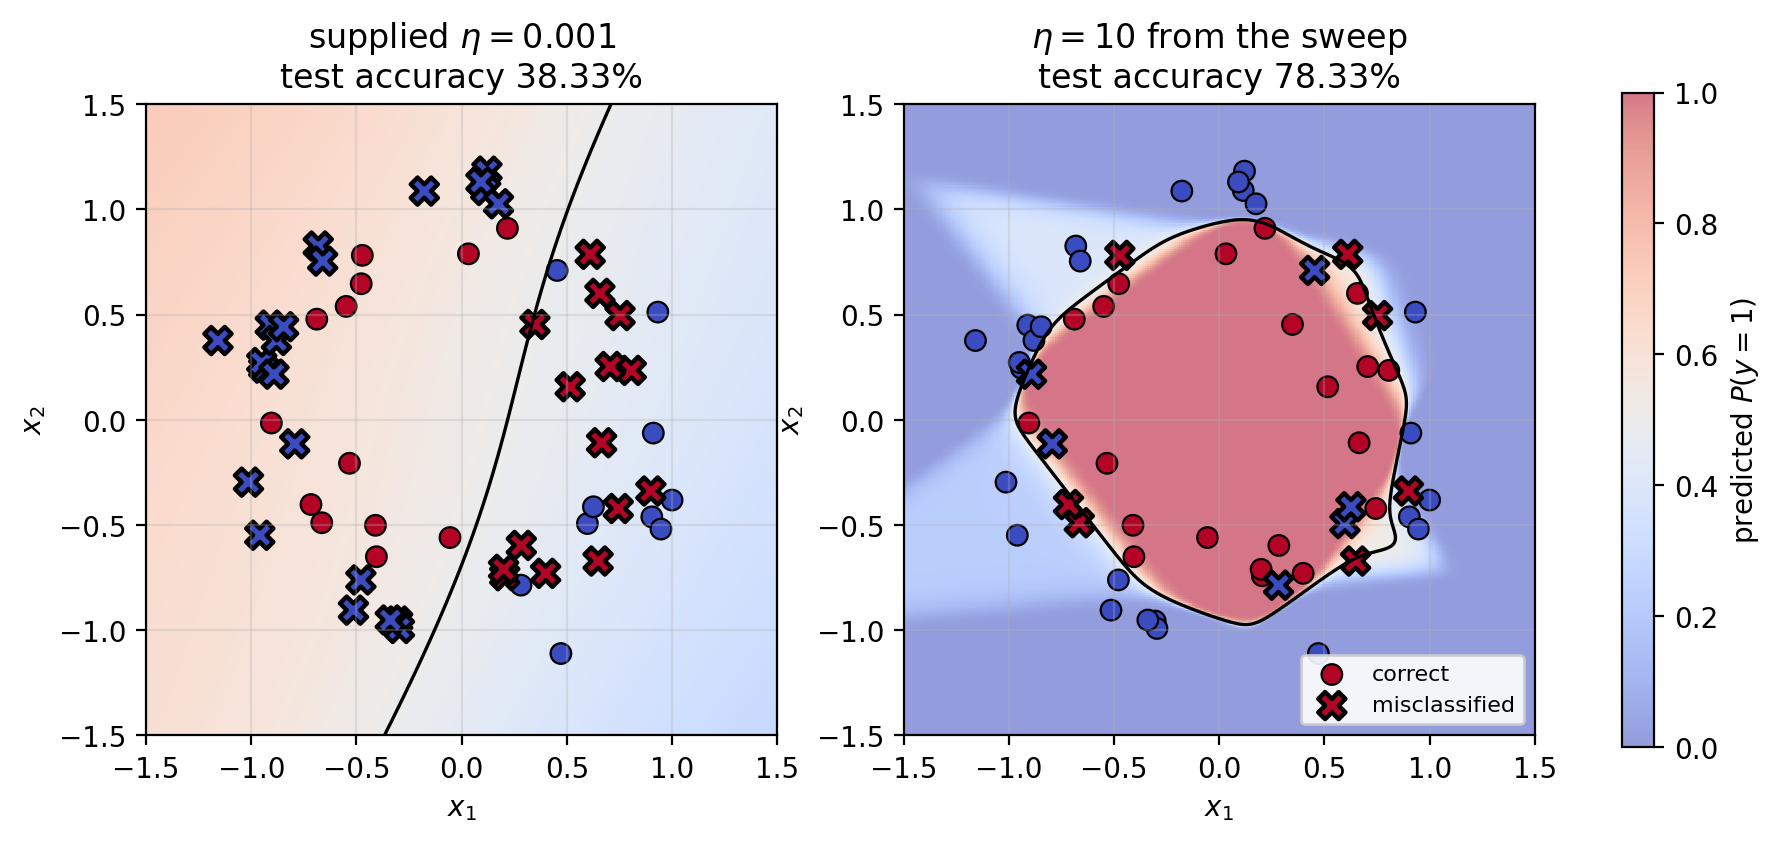
\includegraphics[width=\textwidth]{figures/p1_1_test_classification.png}
\caption{Classification of the 60 held-out test points. Background shading is the
predicted probability $P(y=1)$ and the black line the $0.5$ decision boundary; circles
are correctly classified test points and crosses misclassified ones. Left: the
learning rate supplied in the test snippet, where the network has not moved away from
its initialisation. Right: the same code and seed at
$\eta=10$, which recovers the circular
boundary.}
\label{fig:p11}
\end{figure}

\subsection{Bayesian optimization of \code{learning\_rate} and \code{alpha}
(7 points)}

\paragraph{An assumption that has to be stated first.} The problem asks for the
best \code{learning\_rate} and \code{alpha}, but the supplied \code{MLP} class
defines no training hyperparameter called $\alpha$. The only \code{alpha} anywhere
in \code{mlp.py} is \code{plt.pcolormesh(..., alpha=0.5)} in the test snippet,
which sets the opacity of the decision-surface shading and has nothing to do with
training. Since the task is to optimise a hyperparameter the code does not yet
contain, some interpretation is unavoidable, and I have made mine explicit rather
than leaving it implied: \textbf{I take $\alpha$ to be the coefficient of an $L_2$
penalty on the network weights}, the standard meaning of \code{alpha} in
\code{scikit-learn}'s \code{MLPClassifier} and in ridge regression, and the
reading under which the search in this section is a meaningful exercise. The
extension is backward-compatible: $\alpha=0$ recovers the supplied unregularised
model exactly, so nothing in Section~1.1 is affected. Should the intended meaning
have been different (a momentum coefficient, say, or a learning-rate decay), the
optimisation machinery below transfers unchanged; only the second coordinate of the
search space would need reinterpreting. I use an $L_2$ penalty
on the weights, leaving the biases unpenalised:
\begin{equation}
J \;=\; L \;+\; \frac{\alpha}{2}
\Big(\lVert W_1\rVert_F^2+\lVert W_2\rVert_F^2\Big).
\end{equation}
The penalty contains no forward-pass quantity, so it adds to the gradient independently
of backpropagation:
$\partial\big(\tfrac{\alpha}{2}\sum W^2\big)/\partial W_{jk} = \alpha W_{jk}$,
hence
\begin{equation}
\nabla_{W_2}J = Z_1^{\top}\delta_2+\alpha W_2,
\qquad
\nabla_{W_1}J = X^{\top}\delta_1+\alpha W_1,
\end{equation}
with the bias gradients unchanged. Biases are excluded because a bias shifts the
decision boundary without controlling how sharply the network responds to its inputs,
so penalising it biases the model toward predicting $0.5$ without reducing capacity.
The coefficient defaults to zero, so every result in Section~1.1 is the unregularised
model. The regularised gradient was checked the same way as before: maximum relative
error $8.62\times 10^{-9}$ against central differences
and $1.11\times 10^{-16}$ against autograd.

\paragraph{Objective.} Two quantities are kept distinct throughout. $L_{cv}$ is the
mean three-fold cross-validated binary cross-entropy on the training partition, and
$g=\log_{10}L_{cv}$ is the transformed value the optimiser minimises. The choices
behind this objective are as follows. Validation \emph{loss} rather than accuracy is
used because accuracy on the 46--47 validation points of a fold is a step function of
the hyperparameters, which a Gaussian process cannot model usefully. Cross-validation is
performed on the training partition only, so the 60 test points are used exactly once.
A fixed initialisation seed per fold makes the objective deterministic in
$(\eta,\alpha)$. The $\log_{10}$ transform prevents divergent configurations from
dominating the surrogate as outliers, and configurations whose weights become
non-finite are recorded at a common cap of $L_{cv}=10$. The search box is
logarithmic, $\log_{10}\eta\in[-3,1]$ and $\log_{10}\alpha\in[-6,0]$, because
Table~\ref{tab:lrsweep} shows the usable band spans four orders of magnitude.

\paragraph{Algorithm.} The surrogate is a Gaussian process with a Mat\'ern
$\nu=5/2$ kernel and a separate length scale per dimension. Their upper bound is
capped at 10: the box is only $4\times6$ units wide in log space, so a length scale of
10 already represents an almost linear trend, and permitting larger values allows the
process to declare a dimension irrelevant and stop searching it. Candidates are scored
by Expected Improvement, which for minimisation is
\begin{equation}
\mathrm{EI}(x) = \big(g^{*}-\mu(x)-\xi\big)\Phi(Z) + \sigma(x)\varphi(Z),
\qquad
Z = \frac{g^{*}-\mu(x)-\xi}{\sigma(x)},
\end{equation}
with $g^{*}$ the best value observed so far, $\mu$ and $\sigma$ the posterior mean
and standard deviation, and $\xi=0.01$ an exploration margin. Each iteration maximises
$\mathrm{EI}$ over 4096 Sobol candidates and refines the best with L-BFGS-B. The
budget is 16 Sobol initial points followed by 34 guided iterations;
Figure~\ref{fig:p12conv} traces both searches.

\paragraph{Result.} The search selects
$\eta = 2.223$ and
$\alpha = 3.75\times 10^{-4}$, with
$g = -0.3712$, that is $L_{cv} = 0.4254$, in
324\,s. Table~\ref{tab:final} shows the effect of tuning
on the held-out test set and Figure~\ref{fig:p12tuned} the decision boundary it
produces.

\begin{table}[H]
\centering
\caption{Models retrained on all 140 training points and evaluated once on the 60 held-out test points.}
\label{tab:final}
\begin{tabular}{lrrrrr}
\toprule
configuration & $\eta$ & $\alpha$ & train acc. & test acc. & test BCE \\
\midrule
supplied defaults & 0.001 & 0 & 55.00\% & 38.33\% & 0.7403 \\
Bayesian optimization & 2.223 & $3.75\times 10^{-4}$ & 86.43\% & 78.33\% & 0.4518 \\
random search & 1.247 & $4.30\times 10^{-4}$ & 85.71\% & 80.00\% & 0.4445 \\
\bottomrule
\end{tabular}
\end{table}

\begin{figure}[H]
\centering
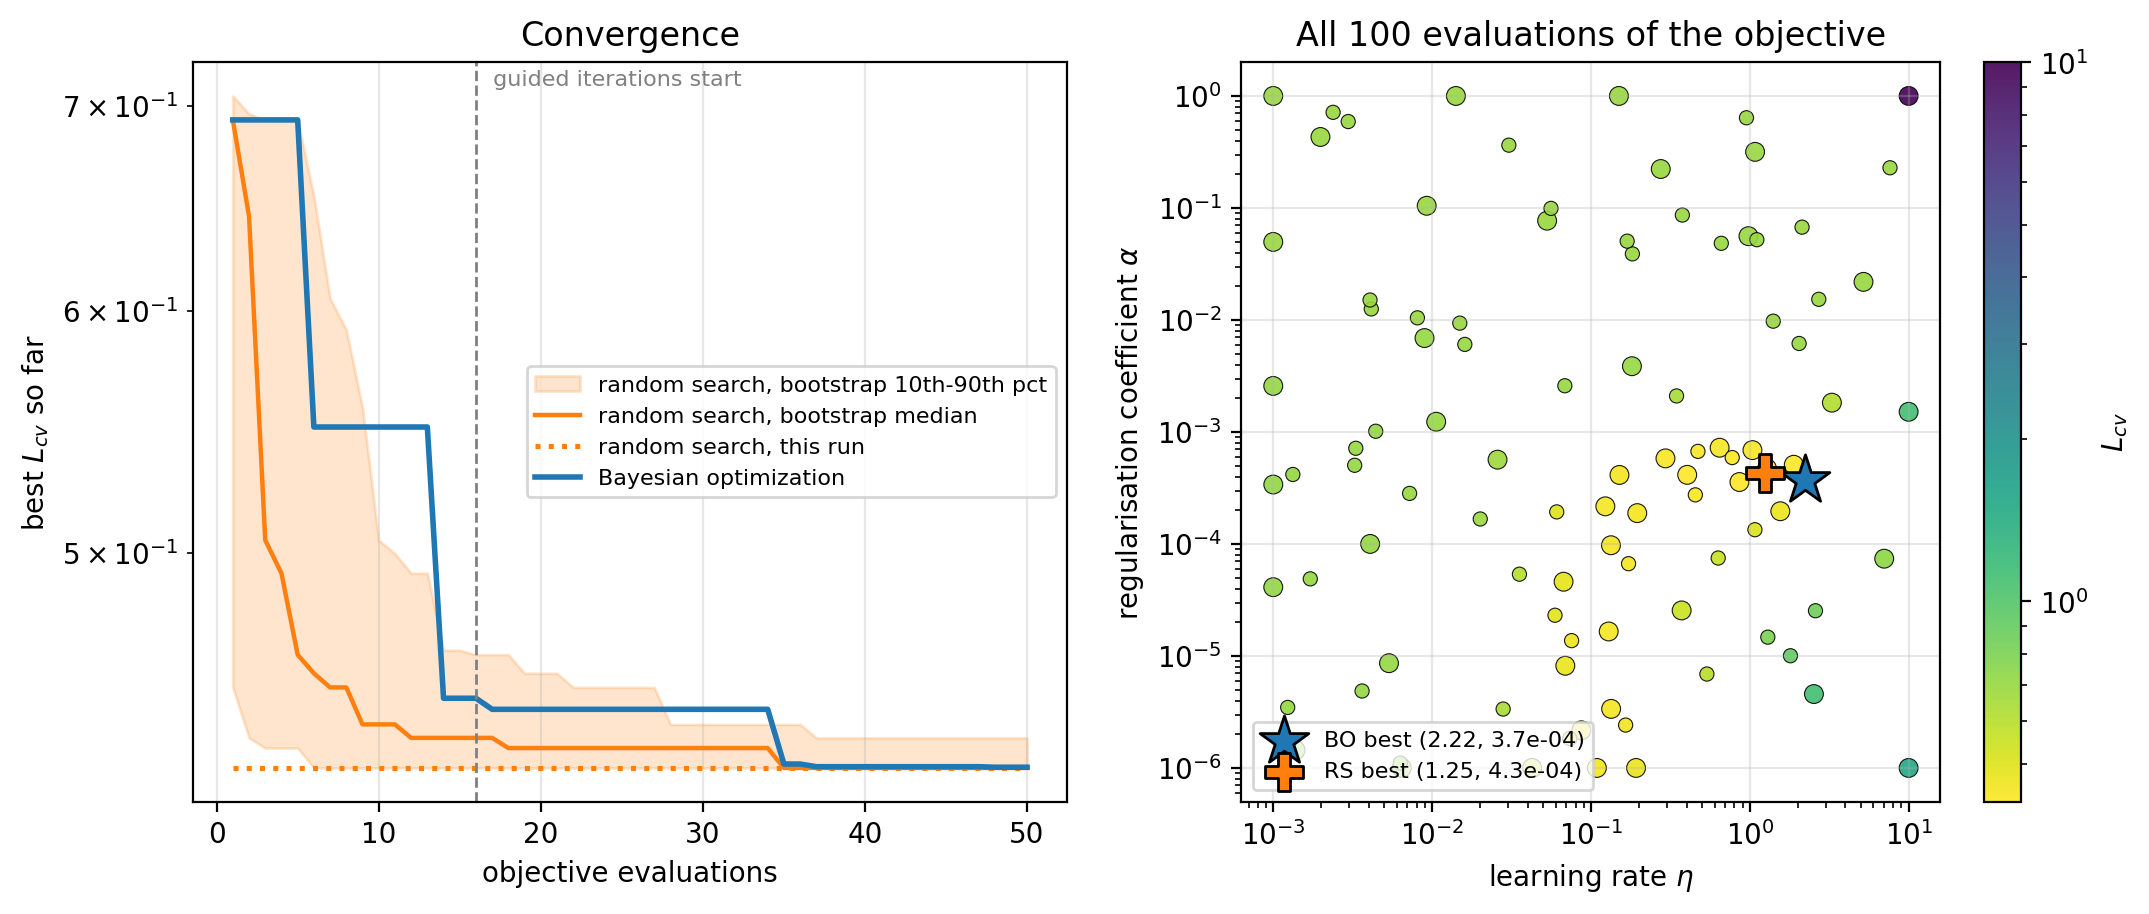
\includegraphics[width=\textwidth]{figures/p1_2_bo_convergence.png}
\caption{Left: best $L_{cv}$ found so far against the number of objective
evaluations. The shaded band is the bootstrap 10th--90th percentile of random
search's best-of-$k$, resampled from its 50 independent draws. The first 16 Bayesian
-optimization evaluations form a Sobol design and are not yet guided. Right: all 100
evaluations from both searches in the $(\eta,\alpha)$ plane, coloured by $L_{cv}$.}
\label{fig:p12conv}
\end{figure}

\paragraph{Comparison with random search.} An uninformed search of the same size,
on the same objective and the same log-scaled box, reaches
$L_{cv} = 0.4252$ at
$\eta=1.247$,
$\alpha=4.30\times 10^{-4}$. The two best values differ by
0.06\,\%, so on final quality the methods are equivalent here. They are
not, however, equally economical with their budget:
16 of the 50 Bayesian evaluations landed in the low-loss region against
6 of the 50 random draws, and 15 of those
16 came from the 34 guided iterations, only 1 from the
16-point Sobol initialisation. The surrogate therefore did steer the search. It simply
had little to gain: the low-loss region occupies a large share of a two-dimensional
box, so 50 random draws are very likely to find it. The advantage of Bayesian
optimization would grow with the dimension of the search space and with the cost of
each evaluation.

\paragraph{What the low-loss region constrains.} Rearranging the update as
$W\leftarrow(1-\eta\alpha)W-\eta\nabla_W L$ suggests that the product $\eta\alpha$
might be the controlling quantity. The evaluations do not support this. The low-loss
set separates into two clusters, one at $\eta\approx0.1$ with $\alpha$ effectively
zero and a better one at larger $\eta$ with $\alpha$ of order $10^{-4}$; within
the better cluster (Table~\ref{tab:spread}) $\alpha$ varies by only
1.33$\times$ while the product varies by
1.90$\times$. Regressing
$\log_{10}\alpha$ on $\log_{10}\eta$ within that cluster gives a slope of
$-0.053$ with
$R^2=0.012$, whereas a constant product would require a
slope of exactly $-1$. The correct statement is therefore that $\alpha$ is pinned to a
narrow band while $\eta$ is only loosely constrained, and that raising $\alpha$ from
nearly zero to about $4\times10^{-4}$ shifts the best learning rate from roughly
$0.1$ to roughly $1$. The two hyperparameters do interact, which is what justifies
searching them jointly, but not through a constant product.

\begin{table}[H]
\centering
\caption{Spread of each candidate invariant across the low-loss evaluations in basin~B. The quantity with the smallest spread is the one the good region actually constrains.}
\label{tab:spread}
\begin{tabular}{lrr}
\toprule
quantity & s.d. of $\log_{10}$ & spread factor \\
\midrule
\code{log10(eta)} & 0.263 & 1.83$\times$ \\
\code{log10(alpha)} & 0.124 & 1.33$\times$ \\
\code{log10(eta*alpha)} & 0.278 & 1.90$\times$ \\
\bottomrule
\end{tabular}
\end{table}

\paragraph{What the penalty does.} Because the decay term acts at every one of the
20\,000 steps, $(1-\eta\alpha)^{T}$ is tempting to read as a cumulative shrinkage
factor. Table~\ref{tab:decay} shows that reading is wrong. The weights start at
$\lVert W\rVert_{\text{init}}=4.73$; at $\alpha=6\times 10^{-4}$, the
setting with the lowest test cross-entropy in the table, pure decay predicts a final
norm of $2.9\times 10^{-5}$ while the measured norm is 19.70, a
discrepancy of about 6 orders of magnitude, and in the opposite
direction, since
the weights have grown rather than shrunk. The prediction fails because the data
gradient is applied at every step as well, so the two forces balance at
$\nabla_W L+\alpha W=0$ instead of compounding. What $L_2$ provides here is a brake on
weight growth. Unregularised training inflates the weight norm to
50.6, saturating the output sigmoid, and cross-entropy
penalises confident errors heavily; at $\alpha=3\times10^{-4}$ the norm settles at
23.6 and the test cross-entropy improves substantially.
An order of magnitude more, and the brake dominates: the norm collapses and the
network can no longer represent a circular boundary.

\begin{table}[H]
\centering
\caption{Effect of the penalty at fixed $\eta=1.0$. The pure-decay column is $\lVert W\rVert_{\text{init}}e^{-T\eta\alpha}$, which the measurement contradicts by many orders of magnitude.}
\label{tab:decay}
\begin{tabular}{lrrrr}
\toprule
$\alpha$ & $\lVert W\rVert$ measured & pure-decay prediction & test acc. & test BCE \\
\midrule
0 & 50.59 & 4.73 & 81.67\% & 0.6701 \\
$1.0\times 10^{-5}$ & 46.55 & 3.87 & 83.33\% & 0.6520 \\
$3.0\times 10^{-5}$ & 41.40 & 2.59 & 83.33\% & 0.5905 \\
$1.0\times 10^{-4}$ & 31.30 & 0.64 & 83.33\% & 0.4899 \\
$3.0\times 10^{-4}$ & 23.59 & 0.0117 & 80.00\% & 0.4561 \\
$6.0\times 10^{-4}$ & 19.70 & $2.9\times 10^{-5}$ & 78.33\% & 0.4535 \\
$1.0\times 10^{-3}$ & 13.80 & $9.7\times 10^{-9}$ & 71.67\% & 0.5440 \\
$3.0\times 10^{-3}$ & 2.07 & $4.1\times 10^{-26}$ & 40.00\% & 0.7123 \\
\bottomrule
\end{tabular}
\end{table}

\begin{figure}[H]
\centering
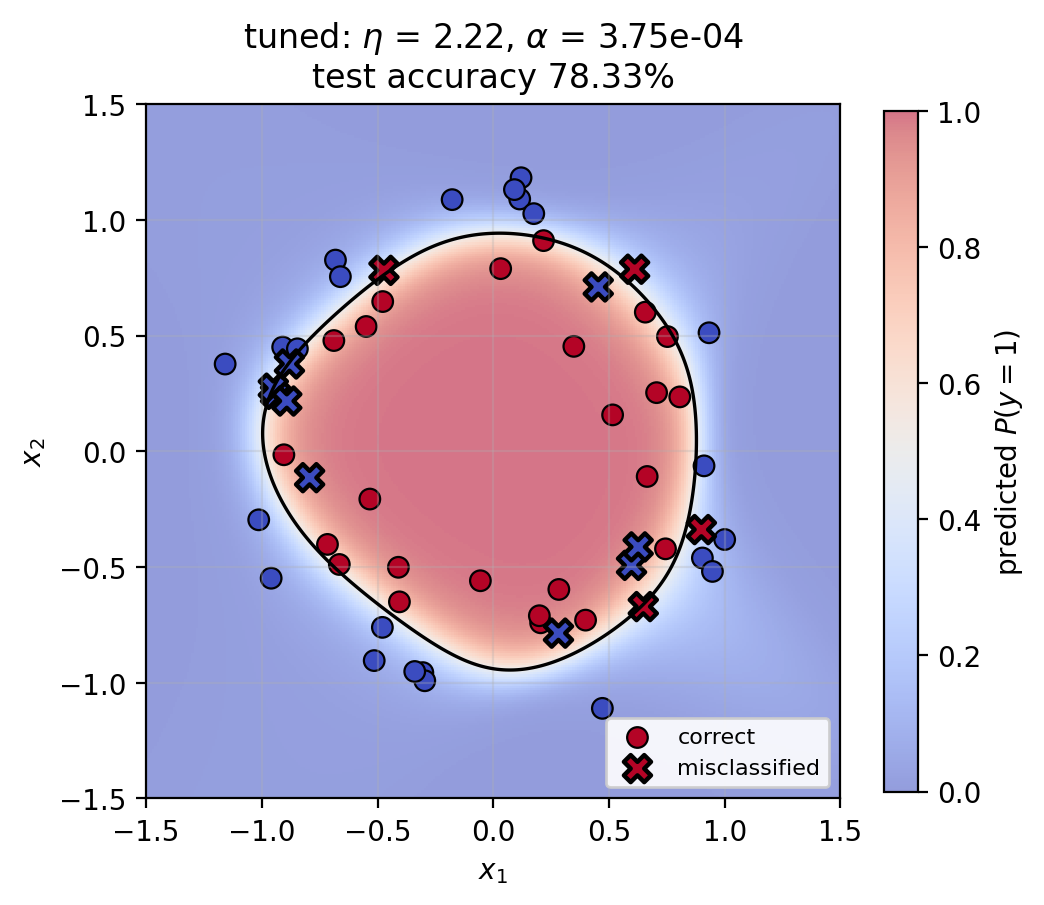
\includegraphics[width=0.55\textwidth]{figures/p1_2_tuned_classification.png}
\caption{Test data classified by the model at the hyperparameters selected by
Bayesian optimization, on the same axes as Figure~\ref{fig:p11}.}
\label{fig:p12tuned}
\end{figure}

\paragraph{Limitations.} Two are worth stating. First, the objective is
cross-entropy, so the selected model is the best calibrated one rather than the most
accurate: an unregularised model at $\eta=1$ reaches a slightly higher test accuracy
while scoring a much worse cross-entropy. Second, the comparison rests on one
Bayesian run against one random-search run; the bootstrap characterises the
distribution of random search but not of Bayesian optimization, so the comparison is
indicative rather than a significance test.

\section{Problem 2 (25 points)}

The task is to forecast pickup and drop-off demand over the next four 15-minute
steps, that is a one-hour horizon. Ten locations are observed over
17664 quarter-hour slots from May to October 2023. Because
the locations move together (the mean pairwise correlation of the pickup series
is $0.68$) and pickups and drop-offs within a
location correlate at $0.70$ on average, the
problem is treated as a single \textbf{system-wide multivariate} forecast: one
model reads all 20 demand channels and predicts all 20 channels at each of the four
future steps, giving 44 input features per time step and
$4\times10\times2=80$ outputs.

\subsection{Cleansing, Dataset class and the split (5 points)}

\paragraph{Cleansing.} Of the 176719 supplied rows,
79 carry timestamps outside the
May--October 2023 study period stated in the problem and are excluded on that
basis; no claim is made about their origin. The remaining
176640 rows contain no duplicate
\code{(datetime, location\_id)} keys and no negative, non-integer or infinite
demand, so nothing else is removed on validity grounds. Extreme values are
deliberately \emph{retained}: the largest counts occur on weekday evenings and are
genuine peak demand, which is exactly the behaviour a fleet-management forecast
exists to capture.

\paragraph{Two different defects.} A row can exist while its demand columns are
empty, so timestamp completeness and value completeness are audited separately.
Comparing the expected grid of $184\times96=
17664$ slots against the observed timestamps of each
location gives zero defects: every row is present. What is missing is the
\emph{value} on 5814 of the
353280 demand entries
(1.6457\%), always in both columns of a row at once, in
runs of at most sixteen slots.

\paragraph{Why entries are masked rather than windows dropped.} Per-channel
missingness is small, but a multivariate window needs all 20 channels at every step,
so the rates compound: 9.86\% of
timesteps have at least one channel missing. Requiring a fully observed input
\emph{and} target window therefore retains only about $70\%$ of samples at a
three-hour lookback and around $1\%$ at a one-day lookback. Masking individual
target entries instead costs 1.6457\% of the supervision.
The adopted rule is:
\begin{itemize}[nosep]
  \item \textbf{inputs} are completed by causal forward fill, which copies from an
    \emph{earlier} timestamp only, plus a per-channel indicator flagging that the
    value was filled. Bidirectional interpolation is rejected because it would use
    observations later than the timestamp being filled, information that does not
    exist at forecast time. Forward fill also cannot move a value from a later
    partition into an earlier one, so it is safe across split boundaries by
    construction;
  \item \textbf{targets} are never imputed. A per-entry mask removes unobserved
    targets from both the loss and every reported metric, so the model is neither
    trained nor scored against a fabricated value.
\end{itemize}

\paragraph{Features and scaling.} Each time step carries 20 standardised demand
channels, 20 imputation flags, and four cyclical calendar terms
$\sin,\cos(2\pi\,\text{tod}/96)$ and $\sin,\cos(2\pi\,\text{dow}/7)$, which keep
23:45 adjacent to 00:00. No month feature is used: with six months and a
chronological split, month identity would be of little use and easy to misuse.
Standardisation is per location $\times$ channel, giving 20 mean and
standard-deviation pairs, because channel means span roughly 14 to 60 trips per 15
minutes, and both
statistics are estimated on May--August alone. Applied to the training period the
transform gives mean $0$ and standard deviation $1$ exactly; on validation and test
it gives $-0.08$ and $+0.16$ respectively, which is the expected behaviour and
confirms that no test information entered the fit.

\paragraph{Dataset class.} \code{TaxiDemandDataset} receives every array through
its constructor and stores only window indices, so \code{\_\_getitem\_\_} performs
slicing and nothing else. One item is
\begin{center}
\code{x}: $(24, 44)$ \quad
\code{y}: $(4, 10, 2)$ \quad
\code{m}: $(4, 10, 2)$, all \code{float32},
\end{center}
with axes (time, feature), (horizon step, location, channel) and the same for the
mask. Demand columns are ordered \code{location\_index}$\times 2+$
\code{channel\_index}. The target is kept in structured form rather than flattened
so that per-horizon and per-location metrics are direct slices.

\paragraph{Split.} The lag-1 autocorrelation of demand is
$0.91$, so a random split
would place near-identical adjacent windows on both sides and leak heavily. The
split is therefore chronological on calendar boundaries, and a sample belongs to the
partition containing its \emph{entire} target horizon; Table~\ref{tab:p2split}
gives the resulting partitions.

\begin{table}[H]
\centering
\caption{Chronological split. A sample is assigned to the partition containing its entire four-step target horizon.}
\label{tab:p2split}
\begin{tabular}{lllr}
\toprule
partition & first target step & last target step & windows \\
\midrule
train & 2023-05-01 06:00:00 & 2023-08-31 23:45:00 & 11,781 \\
val & 2023-09-01 00:00:00 & 2023-09-30 23:45:00 & 2,877 \\
test & 2023-10-01 00:00:00 & 2023-10-31 23:45:00 & 2,973 \\
\bottomrule
\end{tabular}
\end{table}

Input windows may reach back into the preceding partition, because an operator
forecasting at 1 September genuinely holds August observations; this is not target
leakage. 6 windows whose horizon straddled a
boundary were dropped. 10 assertions are
executed in the notebook, covering partition ordering, disjointness of target
timestamps, the requirement that every input step strictly precedes its own targets,
horizon contiguity, and that the scaling statistics were computed from training rows
only. One dataset item was also traced back to the source CSV: de-standardising
\code{y} recovers the four recorded pickup counts exactly.

\subsection{Architecture, training and evaluation (15 points)}

\paragraph{Metrics.} Everything is measured over observed target entries only and
reported in trips per 15 minutes,
\begin{equation}
\text{MAE}=\frac{\sum_i m_i|\hat y_i-y_i|}{\sum_i m_i},\quad
\text{RMSE}=\sqrt{\frac{\sum_i m_i(\hat y_i-y_i)^2}{\sum_i m_i}},\quad
\text{bias}=\frac{\sum_i m_i(\hat y_i-y_i)}{\sum_i m_i} ,
\end{equation}
with squared errors accumulated globally before the square root. MAPE is not used
because many targets are exactly zero. The training loss is the same masked mean
squared error on standardised targets. Both were verified against a hand-computed
example, and setting a masked prediction to $-10^6$ leaves the loss unchanged.

\paragraph{Candidate architectures.} Three models were compared. Their sizes are
not identical (148,752 parameters for the MLP,
83,696 for the CNN and 99,408 for
the LSTM), because flattening makes the MLP's input layer grow with the lookback
while the other two share parameters across time. That works against the conclusion
rather than for it: the MLP is the \emph{largest} of the three and still the weaker
of the two feed-forward options, so its deficit is a matter of inductive bias and not
of capacity. The MLP flattens the window and can mix all lags and channels but has no
temporal structure. The 1-D CNN
convolves along time with dilations $1,2,4$ and kernel $3$, a receptive field of
$1+2(1+2+4)=15$ steps, and shares weights across time. The LSTM keeps a recurrent
state along the sequence. Every model saw identical inputs, samples, mask, optimiser,
batch size, epoch budget and early-stopping rule. The selection criterion, lowest
validation MAE, was fixed before the results were seen.

\paragraph{Choosing the lookback.} Architecture and lookback interact, so they were
chosen in two passes on validation data: the three architectures were compared at a
provisional lookback of 12 steps, the winner was
then swept over lookback, and finally all three were re-compared at the selected
value to check that the ranking still held. The sweep settles on
$L=24$ steps, that is
6 hours of history, ahead of the next best candidate by
0.0694 trips per 15 minutes.

A cheap ridge regression on the flattened window was run first as a deterministic
reference, and it points the other way: it is minimised at the shortest window it was
offered and degrades steadily as the window grows. The disagreement is informative
rather than contradictory. Flattening adds
44 inputs for every extra step, so a linear model pays a
dimension penalty on a fixed number of training samples, and neighbouring windows are
strongly collinear. A recurrent model reuses the same parameters at every step and is
not charged in the same way, so it can exploit sequence length the linear probe
cannot. This is the reason the lookback was ultimately selected with the architecture
that is actually deployed rather than with a cheaper stand-in.

\begin{table}[H]
\centering
\caption{Validation comparison. Baselines have no lookback or parameters. No test metric appears here: the test partition was still sealed at this stage.}
\label{tab:p2arch}
\begin{tabular}{lrrrrr}
\toprule
model & $L$ & parameters & best epoch & val MAE & val RMSE \\
\midrule
Persistence & -- & -- & -- & 8.6235 & 13.1995 \\
Seasonal naive (t-1 week) & -- & -- & -- & 16.6650 & 26.5186 \\
Historical Average & -- & -- & -- & 11.2659 & 18.3915 \\
MLP & 24 & 148752 & 19 & 7.5072 & 10.9590 \\
1-D CNN & 24 & 83696 & 3 & 7.9969 & 11.6808 \\
LSTM & 24 & 99408 & 9 & 6.6798 & 10.1203 \\
\bottomrule
\end{tabular}
\end{table}

\paragraph{Selection.} The LSTM has the lowest validation MAE, and the margin is
not initialisation noise. Repeating the top two architectures over three seeds
(Table~\ref{tab:seeds}) gives a mean validation MAE of 6.7095 for the
LSTM against 7.5536 for the MLP, a gap of
0.8441 trips per 15 minutes against a pooled seed standard
deviation of 0.0405, a ratio of
20.8, so the ordering cannot
be an artefact of initialisation. The selected model is a single recurrent
layer, \code{LSTM}$(44\to128)$, dropout $0.1$, then a linear head to the 80
outputs, reshaped to $(4,10,2)$: 99408 parameters,
matching the closed-form count exactly.

\begin{table}[H]
\centering
\caption{Seed stability of the top two architectures at $L=24$, each retrained from three initialisations. These means, not the single reference-seed run of Table~\ref{tab:p2arch}, are what the selection argument rests on.}
\label{tab:seeds}
\begin{tabular}{lrrrrr}
\toprule
model & seeds & mean val MAE & s.d. & min & max \\
\midrule
LSTM & 3 & 6.7095 & 0.0390 & 6.6798 & 6.7536 \\
MLP & 3 & 7.5536 & 0.0420 & 7.5072 & 7.5890 \\
\bottomrule
\end{tabular}
\end{table}

\paragraph{Training.} Adam at $10^{-3}$, batch size 64, at most 60 epochs, early
stopping on validation masked MSE with patience 8 and the best checkpoint restored,
which occurred at epoch 9. The output head is linear, so
all three architectures emit a small fraction of negative demands; the selected model
is therefore clipped at zero, a rule adopted because it lowered validation MAE. One
consequence has to be stated plainly, because it is easy to miss: every validation
figure in Tables~\ref{tab:p2arch} and~\ref{tab:seeds} is measured
\emph{before} that clipping step, since the clipping rule was only fixed once an
architecture had been chosen, whereas the October figures in
Table~\ref{tab:p2test} are measured \emph{after} it. The two sets of numbers are
therefore not strictly like-for-like, and the small val-to-test difference should not
be read as a generalisation gap measured on a common footing. The whole pipeline was
frozen before the test partition was touched, and October was then evaluated exactly
once (Protocol A: the validation-selected checkpoint, trained on May--August only).

\paragraph{A recording outage in September.} While inspecting errors, a period was
found where recorded demand collapses across all ten locations simultaneously:
331 consecutive slots from 21 to 24 September, with a
missing rate of about 24\,\% against 1.2\,\% elsewhere and a mean observed value near
$1.6$ trips per 15 minutes. It is isolated by a criterion no daily cycle can trigger, namely
a contiguous run of at least 24 hours below 5 trips per 15 minutes,
whereas the longest genuine overnight lull in six months is four hours. The event lies entirely
inside September: the training and test partitions contain
0 and 0 of its slots
respectively, so neither the fitted model nor the October evaluation is affected. The
architecture ranking is unchanged when those validation targets are excluded, so the
selection does not depend on them. The affected values were left in place rather than
removed, and the robustness check is reported instead.

\begin{table}[H]
\centering
\caption{October results, computed once after the pipeline was frozen. Negative bias means the method under-predicts on average.}
\label{tab:p2test}
\begin{tabular}{lrrr}
\toprule
model & test MAE & test RMSE & test bias \\
\midrule
LSTM & 6.6880 & 9.8475 & -0.4760 \\
Persistence & 9.7614 & 14.2695 & -0.0026 \\
Seasonal naive (t-1 week) & 9.7410 & 15.0859 & -1.2891 \\
Historical Average & 8.2766 & 12.5488 & -4.5234 \\
\bottomrule
\end{tabular}
\end{table}

\paragraph{Test results.} On October the selected model reaches a MAE of
6.6880 and an RMSE of 9.8475 trips per 15
minutes, reproduced independently in NumPy. Error grows with the horizon, from
6.4438 at $+15$ minutes to 6.8801 at
$+60$ minutes, which is expected but was measured rather than assumed. After
clipping, no prediction is negative. Figure~\ref{fig:p22curve} shows the training
run behind the restored checkpoint and Figure~\ref{fig:p22example} one October day
of forecasts.

\paragraph{How much the lookback choice is really worth.} The sweep is worth a
caveat. The margin that selected $L=24$ over the
next candidate is 0.0694 trips per 15 minutes,
larger than the seed-to-seed spread of 0.0405 but of the
same order, and it was measured on a single month of validation data that also
contains the September outage discussed above. A margin of that size is enough to
break a tie under a pre-declared rule, which is how it was used, but it is not on its
own strong evidence that six hours of history generalises better than three. Whether
it transfers is not something this experiment can answer: the test partition was
unsealed once, for the selected configuration only, and re-opening it to score the
shorter window would be exactly the kind of test-set selection the protocol exists to
prevent. The point applies to the whole tuning exercise and not just to this one
parameter.

\begin{figure}[H]
\centering
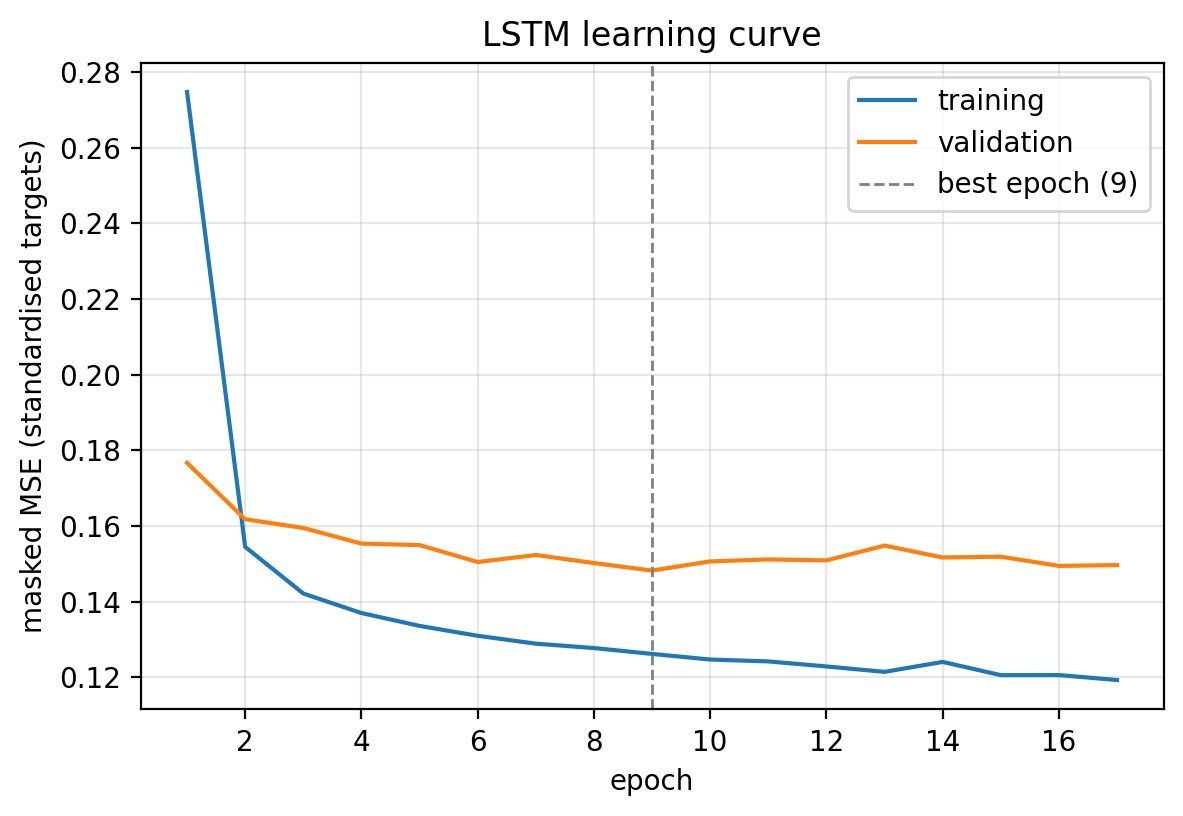
\includegraphics[width=0.72\textwidth]{figures/p2_2_learning_curve.png}
\caption{Training and validation loss for the selected model. The dashed line marks
the checkpoint restored by early stopping.}
\label{fig:p22curve}
\end{figure}

\begin{figure}[H]
\centering
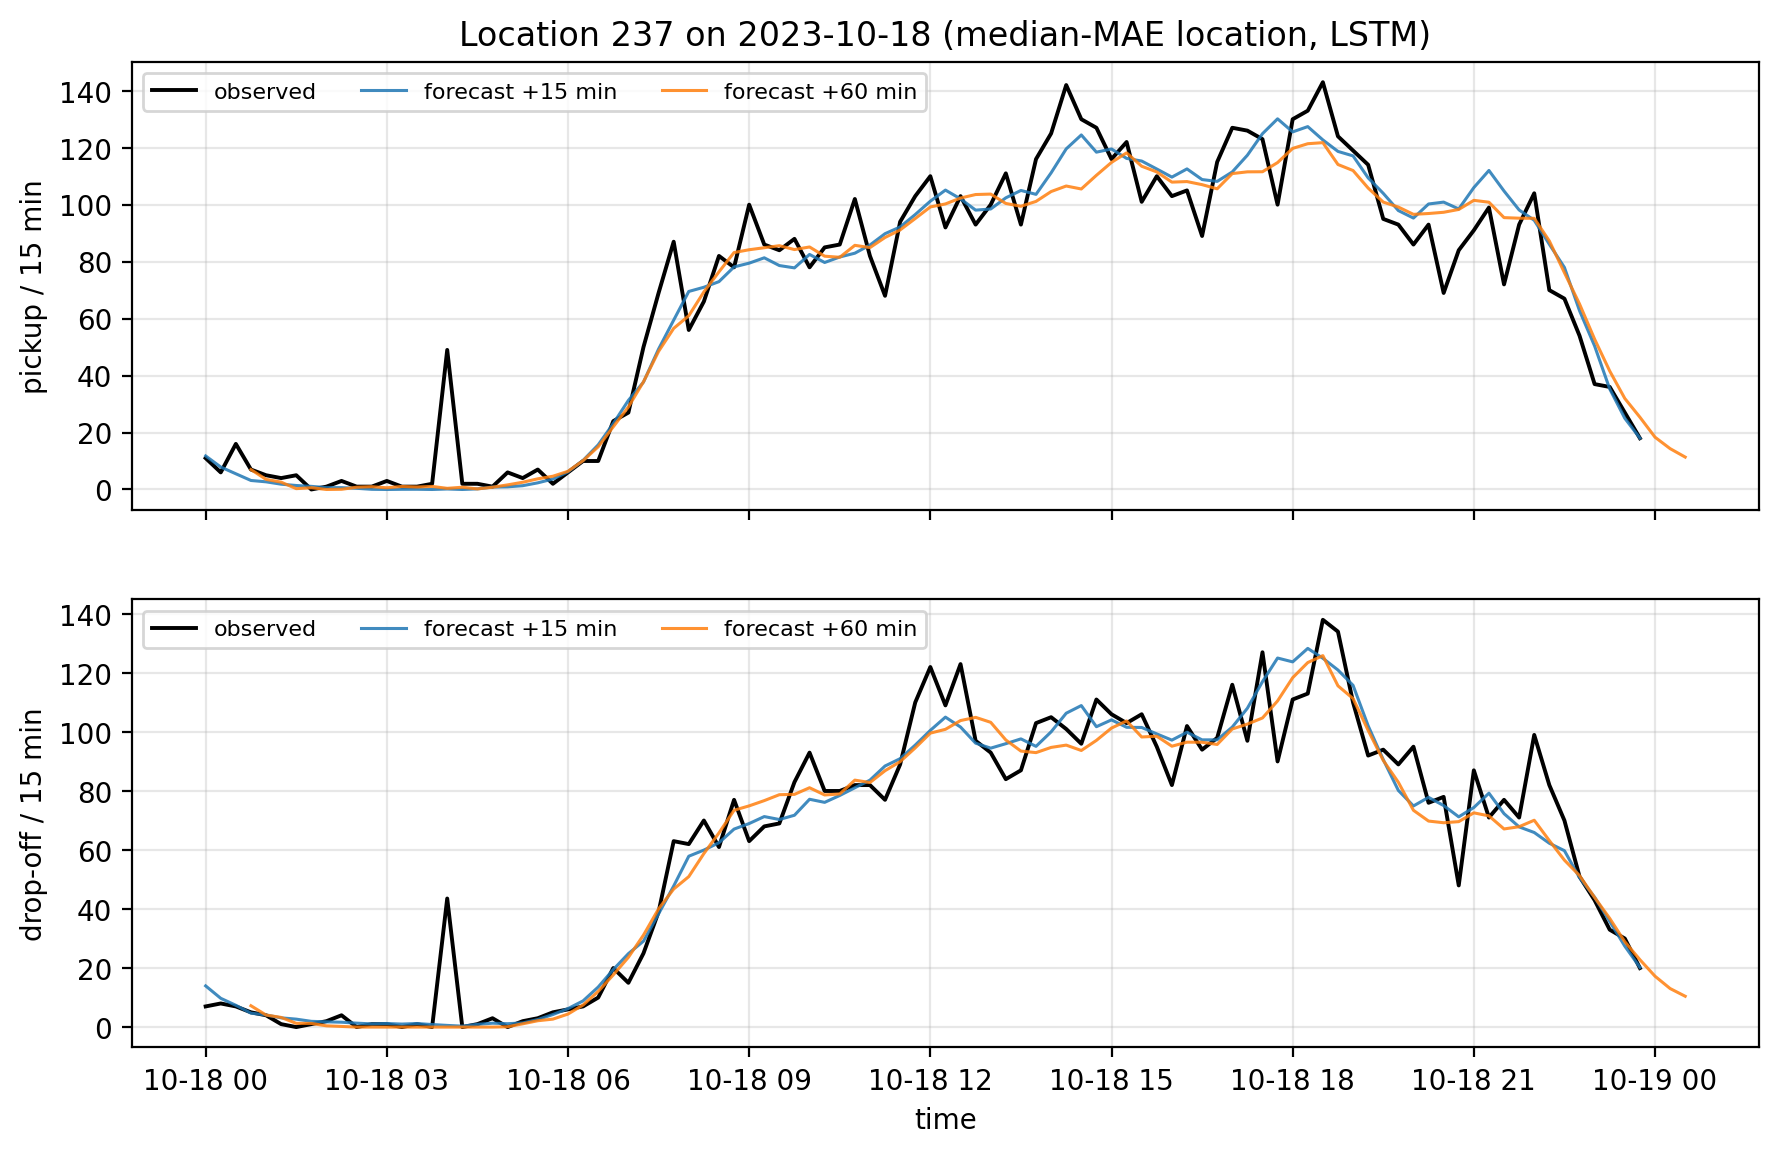
\includegraphics[width=\textwidth]{figures/p2_2_forecast_example.png}
\caption{Observed demand and the $+15$ and $+60$ minute forecasts for one October
day. The location is the one with median test MAE, picked by that rule rather than
for appearance; the day was fixed in advance as a mid-October Wednesday and was not
selected on the results.}
\label{fig:p22example}
\end{figure}

\subsection{Deep learning versus traditional time-series methods (5 points)}

The forecasting problem here has three features that matter for this comparison: the
target is 20 demand channels rather than one series, the ten locations and the two
channels within a location move together, and the whole one-hour horizon has to be
produced at once. A neural network suits that shape. A single LSTM forward pass maps
6 hours of history for all 20 channels, plus the calendar
terms and the imputation flags, onto all $4\times10\times2$ future values, and it can learn
nonlinear relations among those inputs without anyone specifying their functional
form. On October it reached a MAE of 6.6880 against
8.2766 for the Historical Average, the strongest of
the three baselines evaluated, a reduction of about 19\,\% relative to
that baseline. The point is not that statistical methods cannot handle several
series or several steps ahead; VAR-type models and SARIMAX with exogenous regressors
exist. It is that one joint model covers all of it here without specifying a separate
relationship for each of the 20 channels.

Traditional methods keep real advantages on this task. The Historical Average answers
a question an operator can state plainly, namely what demand normally occurs at
this location, on this weekday, at this time, and it needs no iterative fitting, no
architecture choice, no early stopping and no tensor pipeline. ARIMA-family models
come with established diagnostics: stationarity, differencing, seasonal terms and
residual checks are all inspectable, and their assumptions are visible in a way that
an LSTM's hidden state is not. That matters for transport planning, where knowing why
a forecast moved can be worth as much as a slightly lower error. They are also less
data-hungry. Six months at 15-minute resolution sounds like a lot, but consecutive
windows overlap in 23 of their
24 input steps and demand is strongly
autocorrelated at short lags, so the number of effectively independent observations
is far below the window count.

The chronological split makes the trade-off concrete. October's mean pickup demand is
about 11\,\%
above the May--August training level, and the two approaches absorbed that shift very
differently. The Historical Average, being a fixed climatology of the training
months, under-predicted October with a bias of
-4.5234 trips per 15 minutes; the same model had
\emph{over}-predicted the lower-demand September. The LSTM's bias was
-0.4760, roughly
10 times smaller in
magnitude, because it conditions on the most recent
6 hours and therefore tracks the prevailing level instead
of assuming it. Not having an explicit stationarity
assumption is not the same as being immune to distribution shift, but on this
particular shift the recent-history model degraded far less.

The conclusion should be read narrowly. In this experiment the selected LSTM had a
lower test MAE and RMSE than every baseline evaluated, which supports using a joint
nonlinear model for this dataset. It does not show that deep learning is generally
preferable: no ARIMA or SARIMAX model was fitted here, so nothing was measured
against a properly specified seasonal statistical model. Such a model could well be
competitive, and it would come with lower implementation complexity and better
interpretability. What the experiment does support is narrower and still useful:
when 20 correlated series must be forecast jointly over several steps and recent
demand carries most of the signal, a single recurrent model is a reasonable choice,
and the accuracy gain has to be weighed against the extra machinery it requires.

\section{Problem 3 (30 points)}

The network is a $3\times3$ grid of nine states. Every time step Emily must move to
an adjacent node, so the admissible actions at a state are exactly its neighbours and
remaining still is not an option. A move earns the reward of the road taken
($-1$, $-3$ or $-5$ for no, low and high congestion), and arriving at node~3 pays an
additional $+10$. The congestion level of each of the twelve roads was read off
Figure~1 of the problem sheet, matching every edge against the three legend entries
by colour and line style; all twelve were unambiguous. The resulting assignment,
which is the one encoded in the notebook and redrawn in Figure~\ref{fig:p34}, is:
no congestion on 2--3, 4--5 and 8--9; low on 1--2, 2--5, 3--6, 4--7 and 5--8; high
on 1--4, 5--6, 6--9 and 7--8.

Node 3 is treated as terminal, so $v(3)=0$ throughout. The sheet calls it the
destination and pays a one-off arrival bonus, which is only coherent if the episode
ends on arrival.

\subsection{Discounted return of a fixed route (6 points)}

Along $7\to8\to5\to2\to3$ the roads are high (7--8), low (8--5), low (5--2) and none
(2--3), and the final move also collects the bonus, so its reward is $-1+10=+9$. With
$\gamma=0.9$,
\begin{equation}
G=\sum_{k=0}^{3}\gamma^{k}r_{k}
=(-5)+0.9(-3)+0.81(-3)+0.729(+9)
=-5-2.7-2.43+6.561
=-3.5690.
\end{equation}
The return is negative: the $+10$ bonus is discounted by $\gamma^{3}=0.729$ and does
not quite offset the congestion penalties accumulated on the way.

\subsection{Uniform random policy (5 points)}

Knowing nothing about the network, Emily chooses uniformly among the admissible
moves, $\pi(a\mid s)=1/|\mathcal{A}(s)|$ (Table~\ref{tab:p32}). Each move is deterministic, so
$P(s'\mid s,a)=1$ for the intended neighbour and the state transition probability
under the policy coincides with the action probability.

\begin{table}[H]
\centering
\caption{Uniform random policy and the induced transition probabilities at nodes 5, 6 and 9. Moves are deterministic, so the two probabilities coincide.}
\label{tab:p32}
\begin{tabular}{rlccc}
\toprule
state & action & $\pi(a\mid s)$ & $P(s'\mid s,a)$ & $P(s'\mid s)$ \\
\midrule
5 & move to 2 & $1/4$ & 1 & $1/4$ \\
5 & move to 4 & $1/4$ & 1 & $1/4$ \\
5 & move to 6 & $1/4$ & 1 & $1/4$ \\
5 & move to 8 & $1/4$ & 1 & $1/4$ \\
6 & move to 3 & $1/3$ & 1 & $1/3$ \\
6 & move to 5 & $1/3$ & 1 & $1/3$ \\
6 & move to 9 & $1/3$ & 1 & $1/3$ \\
9 & move to 6 & $1/2$ & 1 & $1/2$ \\
9 & move to 8 & $1/2$ & 1 & $1/2$ \\
\bottomrule
\end{tabular}
\end{table}

Node~5 is interior with four neighbours, node~6 is an edge state with three, and
node~9 is a corner with two, which is why the three probabilities differ.

\subsection{Two sweeps of iterative policy evaluation (12 points)}

With $\gamma=1$ and $v_0(s)=0$, the Bellman expectation equation for this policy is
\begin{equation}
v_{k+1}(s)=\sum_{a}\pi(a\mid s)\big[r(s,a)+\gamma v_k(s')\big]
=\frac{1}{|\mathcal{A}(s)|}\sum_{s'\in\mathcal{N}(s)}
\big[r(s,s')+v_k(s')\big].
\end{equation}
The sweeps are synchronous: both use $v_k$ on the right-hand side, so the result does
not depend on the order in which states are visited. Table~\ref{tab:p33} gives the
two sweeps as exact fractions.

\begin{table}[H]
\centering
\caption{Two synchronous sweeps of iterative policy evaluation under the uniform random policy, $\gamma=1$, shown as exact fractions. Node 3 is terminal.}
\label{tab:p33}
\begin{tabular}{rccc}
\toprule
state & $v_0$ & $v_1$ & $v_2$ \\
\midrule
1 & 0 & -4 & -5 \\
2 & 0 & 1 & -4/3 \\
3 & 0 & 0 & 0 \\
4 & 0 & -3 & -20/3 \\
5 & 0 & -3 & -9/2 \\
6 & 0 & -1 & -3 \\
7 & 0 & -4 & -7 \\
8 & 0 & -3 & -19/3 \\
9 & 0 & -3 & -5 \\
\bottomrule
\end{tabular}
\end{table}

As a worked example, the second sweep at node~2 uses the three neighbours 1, 3 and 5
with rewards $-3$, $+9$ and $-3$ and the first-sweep values $v_1(1)=-4$, $v_1(3)=0$
and $v_1(5)=-3$:
\begin{equation}
v_2(2)=\tfrac{1}{3}\big[(-3-4)+(9+0)+(-3-3)\big]
=\tfrac{1}{3}(-7+9-6)=-\tfrac{4}{3}\approx-1.3333.
\end{equation}
After one sweep only node~2 has a positive value, because it is the sole state from
which the bonus is reachable in a single move. After the second sweep every value has
fallen, since one sweep of a random walk mostly accumulates further congestion
penalties; the states nearest the charging station remain the least negative.

\subsection{Greedy policy and its optimality (7 points)}

Acting greedily with respect to $v_2$ (Figure~\ref{fig:p34}) means taking
$\arg\max_a\big[r(s,a)+v_2(s')\big]$ at each state, which gives
$1\to2$, $2\to3$, $4\to5$, $5\to2$, $6\to3$, $7\to4$, $8\to9$ and $9\to8$.

\begin{figure}[H]
\centering
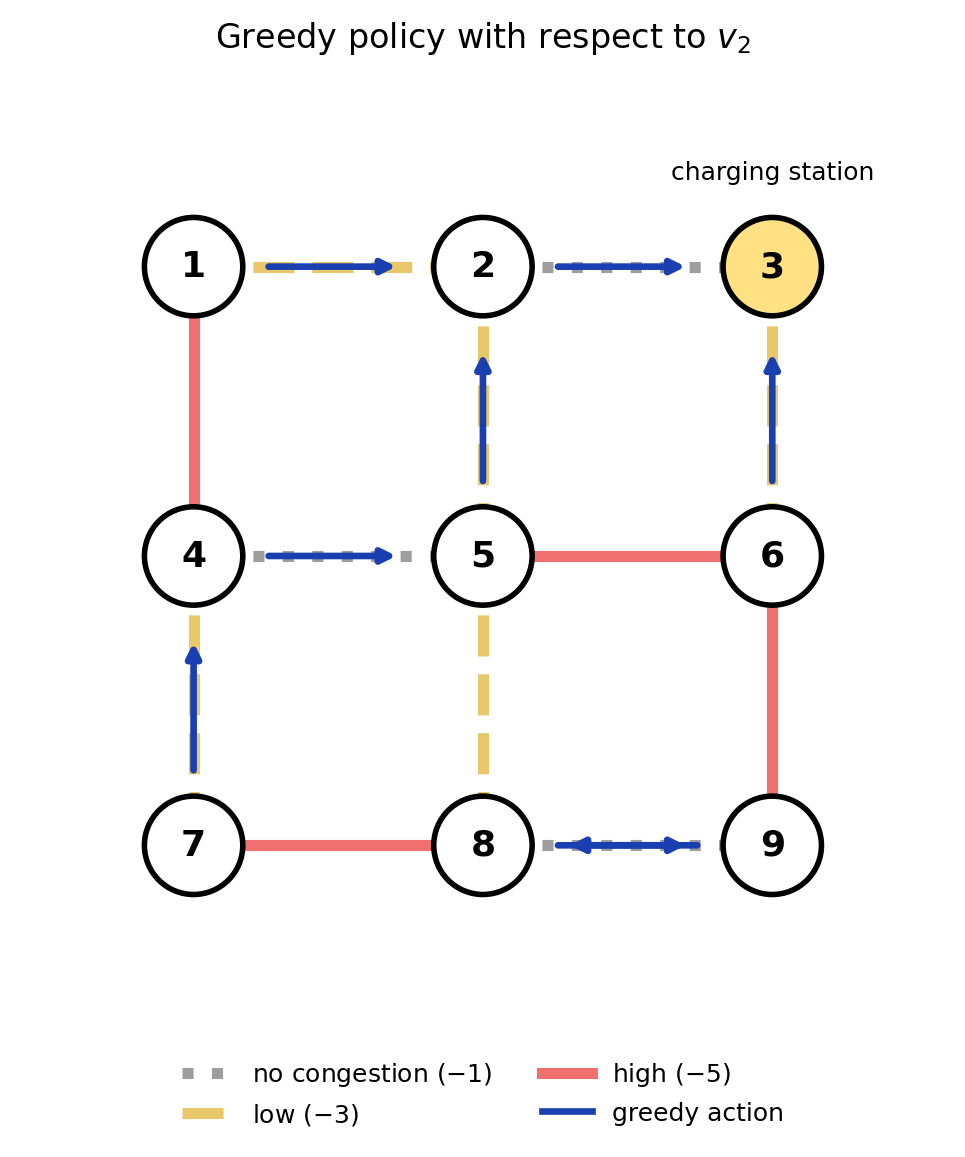
\includegraphics[width=0.58\textwidth]{figures/p3_4_greedy_policy.png}
\caption{The greedy policy with respect to $v_2$. Edge colour and style show the
congestion level; arrows show the chosen move. Nodes 8 and 9 point at each other.}
\label{fig:p34}
\end{figure}

\paragraph{It is not the optimal policy.} Running value iteration to convergence
gives $v^{*}=(6,9,0,5,6,7,2,3,2)$ for states 1 to 9 and the optimal actions
$1\to2$, $2\to3$, $4\to5$, $5\to2$, $6\to3$, $7\to4$, $8\to5$ and $9\to6$ or
$9\to8$. The greedy policy agrees everywhere except at node~8. There the successor
value actually favours node~5, since $v_2(5)=-9/2$ is above $v_2(9)=-5$, but the
greedy rule scores the whole move rather than the destination alone, and the road
8--9 is uncongested while 8--5 carries low congestion. The cheaper edge more than
covers the gap in successor value:
$-1+v_2(9)=-6$ against $-3+v_2(5)=-7.5$, so $8\to9$ wins by $1.5$. That single
disagreement is
enough to break the policy: 8 points to 9 and 9 points back to 8, so from either
state Emily cycles between them and never reaches the charging station at all. Only
6 of the eight non-terminal states reach the
goal under this policy. The failure is a consequence of truncating the evaluation
after two sweeps, since the values have not yet propagated the fact that node~5 is
close to the bonus, and not a defect of policy iteration itself, which alternates
evaluation and improvement until nothing changes.

\paragraph{Can optimality be guaranteed in practice?} For a finite MDP with known
and exact transition probabilities and rewards, policy iteration is guaranteed to
reach an optimal policy in finitely many steps: each improvement step yields a policy
at least as good, and there are only finitely many deterministic policies. That
guarantee is relative to the model, not to the world. In a real road network the
transitions are not deterministic, since a closure or a queue may prevent the
intended move; congestion is stochastic and varies through the day, so a fixed
reward of
$-5$ for a road is at best an average, and a policy that is optimal at 08:00 need not
be at 22:00. If the rewards or transition probabilities are estimated from data,
their estimation error carries into the solution. The state space also has to stay
small enough to sweep, which a city-scale network is not. And as this exercise shows,
a truncated computation can return a policy that is not merely suboptimal but
non-terminating. Optimality is therefore guaranteed with respect to the assumed model
and a converged computation; both assumptions need checking before the result is
trusted in practice.

\section{Problem 4 (30 points)}

\subsection{Manual convolution (5 points)}

For a $4\times4$ input, a $3\times3$ kernel, stride 1 and no padding the output size
in each dimension is $\lfloor (H-k)/s\rfloor+1=(4-3)/1+1=2$, so the result is
$2\times2$. Each entry is the sum of the elementwise product of $K$ with the
corresponding window. Every window of $I$ consists of three identical rows, either
$(10,10,0)$ or $(10,0,0)$, and $K$ has columns $(+1,0,-1)$, so every row contributes
$10-0=10$ and every window totals $30$:
\begin{equation}
I*K=\begin{pmatrix}30 & 30\\ 30 & 30\end{pmatrix}.
\end{equation}

\paragraph{Convention.} This is cross-correlation, which is what convolutional
layers compute and what the function of Section~4.2 implements. A true mathematical
convolution rotates the kernel by $180^{\circ}$ first; for this $K$ that maps the
columns $(+1,0,-1)$ to $(-1,0,+1)$ and flips the sign of every entry, giving
$-30$ throughout. The magnitude and the
interpretation are unchanged.

\paragraph{What the filter detected.} $K$ subtracts the right column of a window
from the left column, so it measures intensity change along the horizontal axis and
therefore responds to \emph{vertical} edges. The image is bright in columns 1--2 and
dark in columns 3--4, a single vertical edge between them, and the response is large
and positive because the transition runs bright to dark from left to right. The
output is constant down each column because nothing in $I$ varies vertically: the
filter has found one vertical edge running the full height of the image. A filter
tuned to horizontal edges would return zeros everywhere on this input.

\subsection{Convolution from scratch (12 points)}

\code{conv2d(image, kernel, stride=1, padding=0)} is implemented with NumPy array
operations only; no built-in convolution routine is used anywhere in this problem.
The image is zero-padded, a strided view produces every window at once, and a single
\code{einsum} contracts each window against the kernel, giving an output of size
$\lfloor (H+2p-k_h)/s\rfloor+1$ by $\lfloor (W+2p-k_w)/s\rfloor+1$. Passing
\code{kernel[::-1, ::-1]} yields a true convolution instead of a cross-correlation.

Correctness was established in two independent ways. The function reproduces the hand
calculation of Section~4.1 exactly, both conventions. It was also checked against a
deliberately naive quadruple-loop implementation written separately, over
81 combinations of image size, kernel shape,
stride and padding: every output matched the size formula and the largest
disagreement in any entry was $5.3\times 10^{-15}$, which is
floating-point rounding.

\subsection{Applying image filters (8 points)}

\code{skimage.data.astronaut()} supplies a genuine RGB image, $512\times512\times3$,
converted to grayscale with the usual luminance weights
$0.2125R+0.7154G+0.0721B$. Both Sobel kernels were applied with stride 1 and padding
1, which preserves the $512\times512$ resolution. Figure~\ref{fig:p43} shows the
grayscale input beside the two responses.

\begin{figure}[H]
\centering
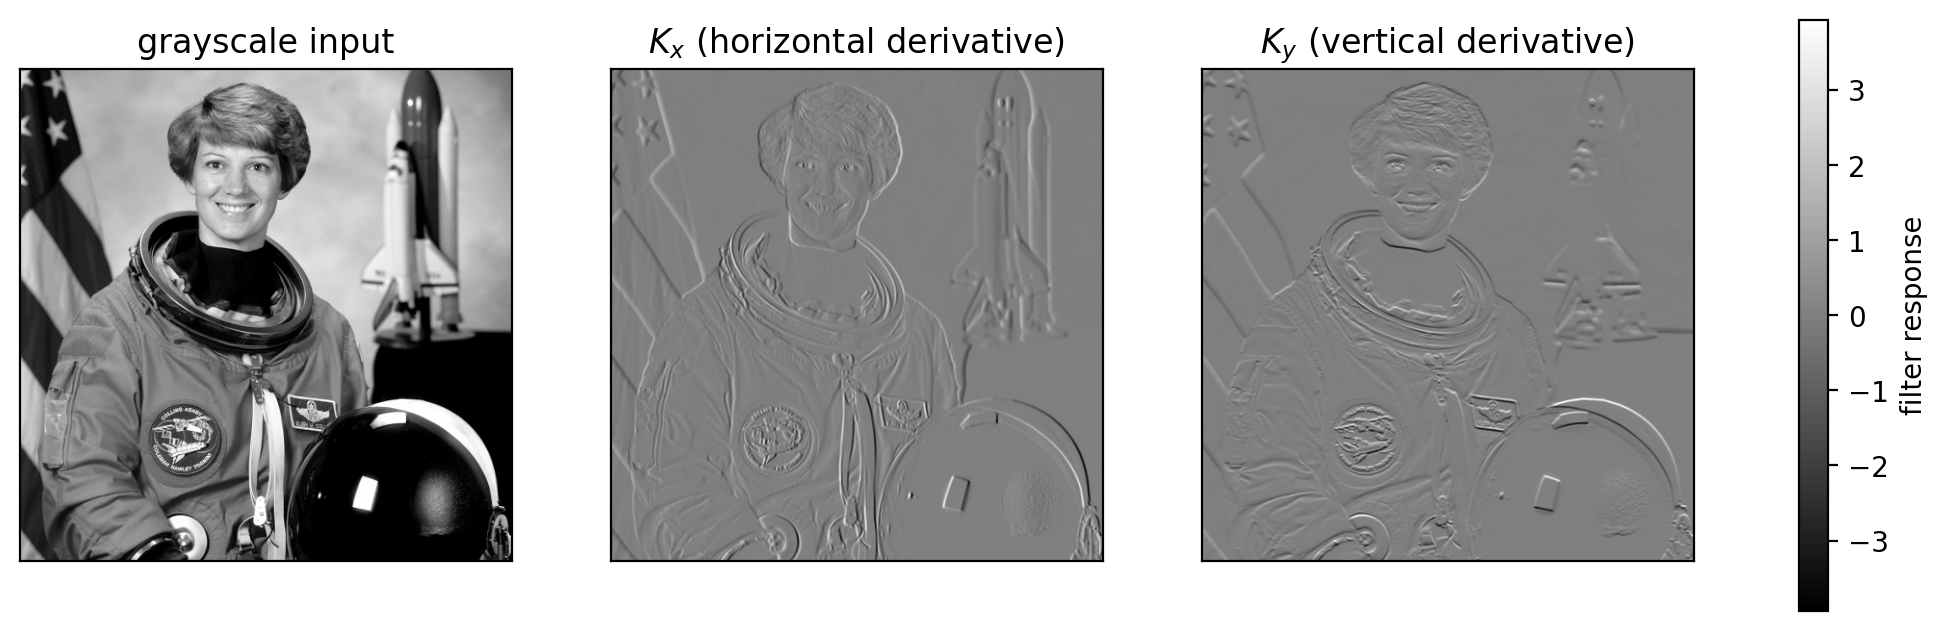
\includegraphics[width=\textwidth]{figures/p4_3_sobel.png}
\caption{Grayscale input and the two Sobel responses on a common symmetric scale.
Mid-grey is a response near zero; light and dark are the two signs of the gradient.}
\label{fig:p43}
\end{figure}

$K_x$ differences the left and right columns of each window, so it responds to
intensity change along the horizontal axis and picks out \emph{vertical} structures: the line
of the shoulder, the upright window frames, the vertical folds of the
suit. $K_y$ differences the top and bottom rows and picks out \emph{horizontal}
structures: the rim of the helmet, the horizontal bands in the background, the
collar. An edge running parallel to a filter's difference direction produces almost
no response, which is why the two maps look close to complementary. On this image the
mean absolute response of $K_x$ is 0.1736 against
0.1441 for $K_y$, consistent with its slightly
stronger horizontal intensity variation.

\subsection{Connection to CNNs (5 points)}

The Sobel kernels above are \textbf{fixed}: their nine weights were chosen by hand
to approximate a first derivative of image intensity, and they are identical for
every image. They encode one specific, human-specified notion of what is worth
measuring.

A convolutional layer performs the same arithmetic (the same sliding window,
elementwise products and sum, the same stride and padding rules implemented in
Section~4.2), but its kernel entries are \textbf{parameters, initialised randomly
and learned by gradient descent}. Each weight receives a gradient of the loss through
backpropagation, exactly as the weights in Problem~1 did, and moves to reduce that
loss. Nobody instructs a kernel to detect edges; if edge detection helps minimise the
training objective then filters resembling Sobel operators tend to appear in the first
layer on their own, and if some other feature is more useful, that appears instead.

Three consequences matter for a task such as image classification. The features are
optimised for the actual objective rather than fixed in advance, so they can capture
structure nobody thought to hand-code. A layer holds many kernels and layers are
stacked, so deeper layers convolve over the feature maps of earlier ones and build a
hierarchy of edges, then corners and textures, then object parts, which would be
impractical to design by hand. And weight sharing keeps this affordable: a $3\times3$
kernel is nine parameters whatever the image size, and the same detector is applied at
every position, so a pattern learned in one part of the image is recognised anywhere
in it. A fully connected layer over a $512\times512$ image would need more than a
quarter of a million weights for a single unit and would have to learn each position
independently.

\end{document}
